% !TeX spellcheck = en_US !TeX root = ../Thesis.tex

In this chapter, we present the module in charge of filtering the input document
and reducing the load of the main algorithm. The plan is to run a light process
that scans the input and quickly finds sections of the document where there is
at least one output. Formally, let $\cA$ be the logical VA constructed from a
REQL query, and let $d$ be a document. For a mapping $\mu$ and a number~$\ell$,
let $\mu_{+\ell}$ be a mapping shifted by $\ell$, namely, for every variable
$x$, $\mu_{+\ell}(x) = \Span{i+\ell}{j+\ell}$ where $\mu(x) = [i, j\rangle$. A
\emph{segmentation} of $d$ is a sequence $[i_1, j_1\rangle, \ldots, [i_k,
j_k\rangle$ of spans of $d$ such that $j_{h} < i_{h+1}$ for every $1 \geq h <
k$. We say that the segmentation is \emph{valid} for $\cA$ over $d$ iff
$$
	\semd{\cA} = \cup_{h=1}^k \{\mu_{+i_h} \mid \mu \in \sem{\cA}(d[i_h, j_h\rangle) \}
$$
namely, if we can evaluate $\cA$ over $d$ by considering the segments $d[i_h,
j_h\rangle$ of $d$ and shifting the results. The task of the filtering module is
to search for a good segmentation that is valid for $\cA$ over $d$,
%and with a computational cost that is considerably lower than running the
%evaluation algorithm over the whole document. 
and which can be computed quickly. Of course, the segmentation $[0, |d|\rangle$
is always valid, and we wish to refine it into smaller segments whenever
possible.
%and then we look for a minimal segmentation whenever it is possible.

Filtering the document into disjoint segments is not new when evaluating regular
expressions. For example, RE2~\citep{cox2007regular} runs a deterministic
automaton back and forth to find the starting and ending positions for the
leftmost-longest match. Unfortunately, such approaches are unsuitable for our
setting. Our approach follows the \emph{split-correctness} framework  proposed
in~\citet{DoleschalKMNN19}. The main goal of split-correctness is to find a REQL
query $\texttt{e}_\cA$ with a single variable such that $\semd{\texttt{e}_\cA}$
is a valid segmentation of $\cA$ over~$d$. The filtering module in \rematch\ is
inspired by split-correctness, but we improve the approach in two ways. First,
\rematch\ does not restrict the filtering module on using single-variable
expressions for finding a segmentation. Instead, for filtering, we consider any
segmentation algorithm (i.e., not necessarily based on a regex) that, given
$\cA$ and $d$, finds a valid segmentation for $\cA$ over $d$. Second, we look
for a ``cheap'' segmentation algorithm, i.e., a process that runs faster than
the evaluation algorithm. Indeed, using RegEx for filtering does not pay off if
computing the segmentation takes longer than evaluating the target query itself.
%Therefore, we want a segmentation procedure that is simple and efficient to
%ensure that it will save time.

%\cristian{Improve here the presentation of the ``light search'' optimization.
%Basically, better present the name of the algorithm. }

\section{Light search (optimization)}

In \rematch, the filtering module finds a segmentation by simulating the logical
VA over the document, but only storing the starting and ending position where
there is at least one output. For this we need the following extension of the
transition relation. Let $\cA = (Q, \delta, q_0, q_f)$ be a logical VA. We
extend $\delta$ to a function $\delta^*$ that given a set $S \subseteq Q$ and a
letter $a$, outputs all states that can be reached from $S$ by using zero or
more variable transitions and then a letter transition that satisfies $a$,
namely, $p \in \delta^*(S,a)$ if there exists a sequence of transitions in
$\delta$ of the form
$
	q \ \trans{v_1} \ q_1 \ \trans{v_2} \ \cdots \ \trans{v_m} \ q_m \ \trans{C} \ p
$
such that $q \in S$, $a \in \cset(C)$, and $v_i$ is a variable marker (e.g.,
$\Open{x}$ or $\Close{x}$) for every $i \leq m$. We also define
$\delta^*(S,\epsilon)$ such that $p \in \delta^*(S,\epsilon)$ if, and only if,
$p$ can be reached from a state in $S$ by only using variable transitions.

\newcommand{\foutput}{\texttt{output}} \newcommand{\fends}{\texttt{ends}}
\newcommand{\fnext}{\operatorname{next}_{\delta}}



\begin{algorithm}[t]
	\caption{[\textsc{Light Search}] The segmentation algorithm for a logical VA
	$\cA = (Q, \delta, q_0, q_f)$ over a document $d = a_0 \ldots
	a_{n-1}$.}\label{alg:segmentation}
	\begin{algorithmic}[1]
		\Procedure{Filtering}{$\cA, a_0 \ldots a_{n-1}$} \State $S \gets
		\emptyset$ \State $i \gets 0, j \gets 0$ \For{$\ell=0$ \textbf{to} $n$}
		\State $(S, \foutput, \fends) \gets \fnext(S, a_\ell)$ \If{$\foutput$}
		\State $j \gets \ell+1$ \ElsIf{$\fends$} \If{$i < j$} \State
		\textbf{Enumerate} $[i, j\rangle$ \EndIf \State $i \gets \ell + 1$
		\EndIf \EndFor \If{$i < j$} \State \textbf{Enumerate} $[i, j\rangle$
		\EndIf \EndProcedure
	\end{algorithmic}
\end{algorithm}

Algorithm~\ref{alg:segmentation}, also called \textsc{Light Search}, presents
the filtering procedure for finding a segmentation of $\cA$ over $d$. The
algorithm simulates $\cA$ over $d$ by keeping a set of states $S \subseteq Q$ of
active runs, namely, each $q \in S$ represents a run of $\cA$ over a prefix of
$d$ that could produce an output. The workhorse of
Algorithm~\ref{alg:segmentation} is the function $\fnext$ (see line 5). Given a
set $S \subseteq Q$ and a letter $a$, the function $\fnext(S, a)$ returns a
triple $(S', \foutput, \fends)$ where $S' \subseteq Q$ and $\foutput, \fends$
are boolean values. The first component $S'$ is equal to $\delta^*(S, a) \cup
\delta^*(\{q_0\}, a)$. Intuitively, $\delta^*(S, a)$ are all states that one can
reach from $S$  by using some variable transitions and reading~$a$. On the other
hand, $\delta^*(\{q_0\}, a)$ are the new states that one can reach by starting
from $q_0$ and reading $a$. Recall that a match can be made from any position in
the document, so we start a fresh run by using $\delta^*(\{q_0\}, a)$. The
second component $\foutput$ is true iff $q_f \in \delta^*(S', \epsilon)$,
namely, $\foutput$ is true when there is a run that reaches the final state.
Finally, $\fends$ is true iff $\delta^*(S, a) = \emptyset$, which tells whether
the runs in $S$ end with the new letter. When implementing
Algorithm~\ref{alg:segmentation} in \rematch, we cache the value of $\fnext(S,
a)$, in order to compute it at most once for every pair $(S,a)$.

We have all the ingredients to explain how Algorithm~\ref{alg:segmentation}
works. The algorithm keeps a set of active states $S$, and two pointers $i$ and
$j$. As we already mentioned, $S$ contains all active states when reading the
document. Instead, the pair $(i, j)$ stores the last span $[i, j\rangle$ (called
active span) where there is an output, namely, $\sem{\cA}(d[i, j\rangle) \neq
\emptyset$. We assume here that, if $j \leq i$, then the algorithm has not found
a segment yet (i.e., from the previous segment that was output). In lines 2-3,
we start by setting $S = \emptyset$ (i.e., no active runs) and $(i,j) = (0,0)$
(i.e., no active span). Then we iterate sequentially over each letter $a_\ell$.
For each letter, we compute $\fnext(S, a_\ell)$ returning the triple $(S',
\foutput, \fends)$ where $S'$ is the new set of active states (line 5). If
$\foutput$ is true, an active state can reach $q_f$ and the segment $[i,
\ell+1\rangle$ contains an output. Then by setting $j = \ell+1$ we update the
new active span (lines 6-7). Instead, if there is no output and $\fends$ is
true, then all active states of the previous iteration end with the new letter
$a_{\ell}$, and we can start a new active span by setting $i = \ell$ (line 11).
However, if $i < j$, then we cannot extend more the active span represented by
$(i,j)$, we can safely return the active span $\Span{i}{j}$ and continue (lines
9-10). Finally, after the document ends (lines 12-13) we check if there is an
active span that was not output (i.e., $i < j$), and return it if this is the
case.

\begin{example}
	In the following figure, we display the execution of
	Algorithm~\ref{alg:segmentation} for the logical VA of query \texttt{e0}
	(see Example~\ref{example:logicalVA}) over the document
	\texttt{thathatsthat}. For each letter, we show below the value of variables
	$\ell$, $S$, $\foutput$, $\fends$, $i$, and $j$ after finishing each
	iteration.

	\vspace{-5mm}
	\begin{center}
		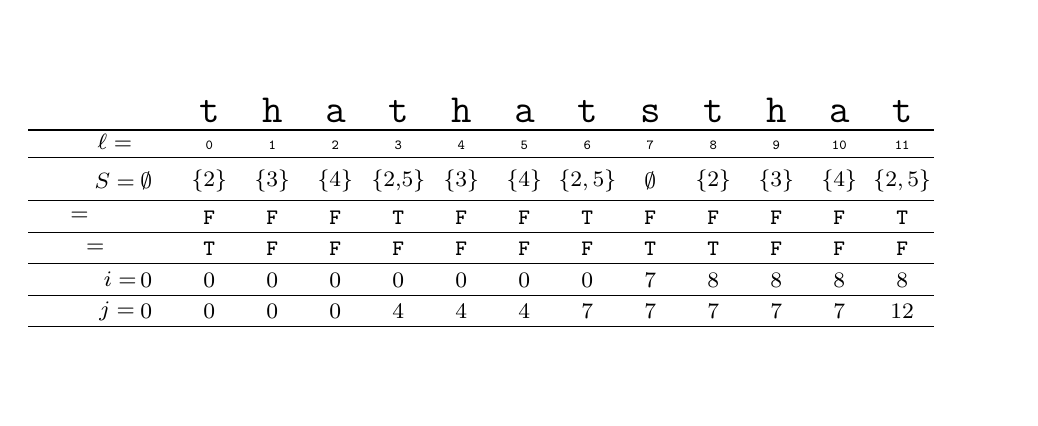
\begin{tikzpicture}[node distance=2cm, every text node
				part/.style={align=center}, lt/.style={outer sep=0mm, inner
				sep=10mm, node distance=8mm, text height=2mm, text centered}]
				\node[lt] (l0) at (0.3,0.3) {\Large \texttt{t}\vphantom{y}};
				\node[lt,right of=l0] (l1) {\Large \texttt{h}\vphantom{y}};
				\node[lt,right of=l1] (l2) {\Large \texttt{a}\vphantom{y}};
				\node[lt,right of=l2] (l3) {\Large \texttt{t}\vphantom{y}};
				\node[lt,right of=l3] (l4) {\Large \texttt{h}\vphantom{y}};
				\node[lt,right of=l4] (l5) {\Large \texttt{a}\vphantom{y}};
				\node[lt,right of=l5] (l6) {\Large \texttt{t}\vphantom{y}};
				\node[lt,right of=l6] (l7) {\Large \texttt{s}\vphantom{y}};
				\node[lt,right of=l7] (l8) {\Large \texttt{t}\vphantom{y}};
				\node[lt,right of=l8] (l9) {\Large \texttt{h}\vphantom{y}};
				\node[lt,right of=l9] (l10) {\Large \texttt{a}\vphantom{y}};
				\node[lt,right of=l10] (l11) {\Large \texttt{t}\vphantom{y}};

			\draw (-2, 0.15) to (9.5, 0.15); {
			\tiny

			\node[lt] (p0) at (0.3,0) {\texttt{0}}; \node[lt,right of=p0] (p1)
			{\texttt{1}}; \node[lt,right of=p1] (p2) {\texttt{2}};
			\node[lt,right of=p2] (p3) {\texttt{3}}; \node[lt,right of=p3] (p4)
			{\texttt{4}}; \node[lt,right of=p4] (p5) {\texttt{5}};
			\node[lt,right of=p5] (p6) {\texttt{6}}; \node[lt,right of=p6] (p7)
			{\texttt{7}}; \node[lt,right of=p7] (p8) {\texttt{8}};
			\node[lt,right of=p8] (p9) {\texttt{9}}; \node[lt,right of=p9] (p10)
			{\texttt{10}}; \node[lt,right of=p10] (p11) {\texttt{11}}; \draw
			(-2, -0.2) to (9.5, -0.2); }

			{
			\footnotesize
			\node at (-0.9,-0) {$\ell = $}; \node[lt] (S0) at (-0.5,-0.5)
			{$\emptyset$}; \node[lt,right of=S0] (S1) {$\{2\}$}; \node[lt,right
			of=S1] (S2) {$\{3\}$}; \node[lt,right of=S2] (S3) {$\{4\}$};
			\node[lt,right of=S3] (S4) {$\{2,\!5\}$}; \node[lt,right of=S4] (S5)
			{$\{3\}$}; \node[lt,right of=S5] (S6) {$\{4\}$}; \node[lt,right
			of=S6] (S7) {$\{2,5\}$}; \node[lt,right of=S7] (S8) {$\emptyset$};
			\node[lt,right of=S8] (S9) {$\{2\}$}; \node[lt,right of=S9] (S10)
			{$\{3\}$}; \node[lt,right of=S10] (S11) {$\{4\}$}; \node[lt,right
			of=S11] (S12) {$\{2,5\}$};

			\node at (-0.9,-0.5) {$S = $};

			\draw (-2, -0.75) to (9.5, -0.75); \node[lt] (O0) at (-0.5,-0.95)
			{}; \node[lt,right of=O0] (O1) {\texttt{F}}; \node[lt,right of=O1]
			(O2) {\texttt{F}}; \node[lt,right of=O2] (O3) {\texttt{F}};
			\node[lt,right of=O3] (O4) {\texttt{T}}; \node[lt,right of=O4] (O5)
			{\texttt{F}}; \node[lt,right of=O5] (O6) {\texttt{F}};
			\node[lt,right of=O6] (O7) {\texttt{T}}; \node[lt,right of=O7] (O8)
			{\texttt{F}}; \node[lt,right of=O8] (O9) {\texttt{F}};
			\node[lt,right of=O9] (O10) {\texttt{F}}; \node[lt,right of=O10]
			(O11) {\texttt{F}}; \node[lt,right of=O11] (O12) {\texttt{T}}; \node
			at (-1.35,-0.95) {$\foutput = $};

			\draw (-2, -1.15) to (9.5, -1.15); \node[lt] (E0) at (-0.5,-1.35)
			{}; \node[lt,right of=E0] (E1) {\texttt{T}}; \node[lt,right of=E1]
			(E2) {\texttt{F}}; \node[lt,right of=E2] (E3) {\texttt{F}};
			\node[lt,right of=E3] (E4) {\texttt{F}}; \node[lt,right of=E4] (E5)
			{\texttt{F}}; \node[lt,right of=E5] (E6) {\texttt{F}};
			\node[lt,right of=E6] (E7) {\texttt{F}}; \node[lt,right of=E7] (E8)
			{\texttt{T}}; \node[lt,right of=E8] (E9) {\texttt{T}};
			\node[lt,right of=E9] (E10) {\texttt{F}}; \node[lt,right of=E10]
			(E11) {\texttt{F}}; \node[lt,right of=E11] (E12) {\texttt{F}}; \node
			at (-1.15,-1.35) {$\fends = $};

			\draw (-2, -1.55) to (9.5, -1.55); \node[lt] (i0) at (-0.5,-1.75)
			{0}; \node[lt,right of=i0] (i1) {0}; \node[lt,right of=i1] (i2) {0};
			\node[lt,right of=i2] (i3) {0}; \node[lt,right of=i3] (i4) {0};
			\node[lt,right of=i4] (i5) {0}; \node[lt,right of=i5] (i6) {0};
			\node[lt,right of=i6] (i7) {0}; \node[lt,right of=i7] (i8) {7};
			\node[lt,right of=i8] (i9) {8}; \node[lt,right of=i9] (i10) {8};
			\node[lt,right of=i10] (i11) {8}; \node[lt,right of=i11] (i12) {8};
			\node at (-0.83,-1.75) {$i = $};

			\draw (-2, -1.95) to (9.5, -1.95); \node[lt] (j0) at (-0.5,-2.15)
			{0}; \node[lt,right of=j0] (j1) {0}; \node[lt,right of=j1] (j2) {0};
			\node[lt,right of=j2] (j3) {0}; \node[lt,right of=j3] (j4) {4};
			\node[lt,right of=j4] (j5) {4}; \node[lt,right of=j5] (j6) {4};
			\node[lt,right of=j6] (j7) {7}; \node[lt,right of=j7] (j8) {7};
			\node[lt,right of=j8] (j9) {7}; \node[lt,right of=j9] (j10) {7};
			\node[lt,right of=j10] (j11) {7}; \node[lt,right of=j11] (j12) {12};
			\node at (-0.87,-2.15) {$j = $};

			\draw (-2, -2.35) to (9.5, -2.35); }
		\end{tikzpicture}
	\end{center}
	\vspace{-10mm}

	\noindent By following the run of the algorithm, we can check that it
	outputs the segmentation $\Span{0}{7}$ and $\Span{8}{12}$ corresponding to
	the substrings \texttt{thathat} and \texttt{that}, respectively.
\end{example}

Algorithm~\ref{alg:segmentation} maintains the invariant that, after reading
$a_\ell$, $i$ is a position before any of the current active runs started and,
if $i < j$,  then $j$ is the latest position such that $\sem{\cA}(d[i, j\rangle)
\neq \emptyset$. Indeed, these invariants are enough to prove that the algorithm
is correct. The following theorem summarizes the correctness of the algorithm
(its proof can be founud in Appendix \ref*{app:segmentation}):

\begin{theorem}\label{theo:segmentation} Given a logical VA $\cA$ and a document
	$d$, Algorithm~\ref{alg:segmentation} outputs a sequence of spans $[i_1,
	j_1\rangle, \ldots, [i_k, j_k\rangle$ that is a valid segmentation for $\cA$
	over $d$.
\end{theorem}

Note that the load of computing Algorithm~\ref{alg:segmentation} is low: we need
one pass over the document and for each letter we need to perform a small number
of simple operations (i.e., apply the function $\fnext$ and check at most two
if-statements). Given that we can cache the output $\fnext(S, a)$ for each new
pair $(S, a)$, the cost per new letter is low when the caching of the function
$\fnext$ stabilizes. This is probably the main reason why filtering runs faster
than performing the main evaluation algorithm (see
Chapter~\ref{chpt:experiments} for further discussion).


